\documentclass{article}
\usepackage{hyperref}
\usepackage{graphicx}

\providecommand{\tightlist}{%
  \setlength{\itemsep}{0pt}\setlength{\parskip}{0pt}}

\begin{document}

\title{Kacper Topolnicki, CV}
\maketitle

\begin{center}
	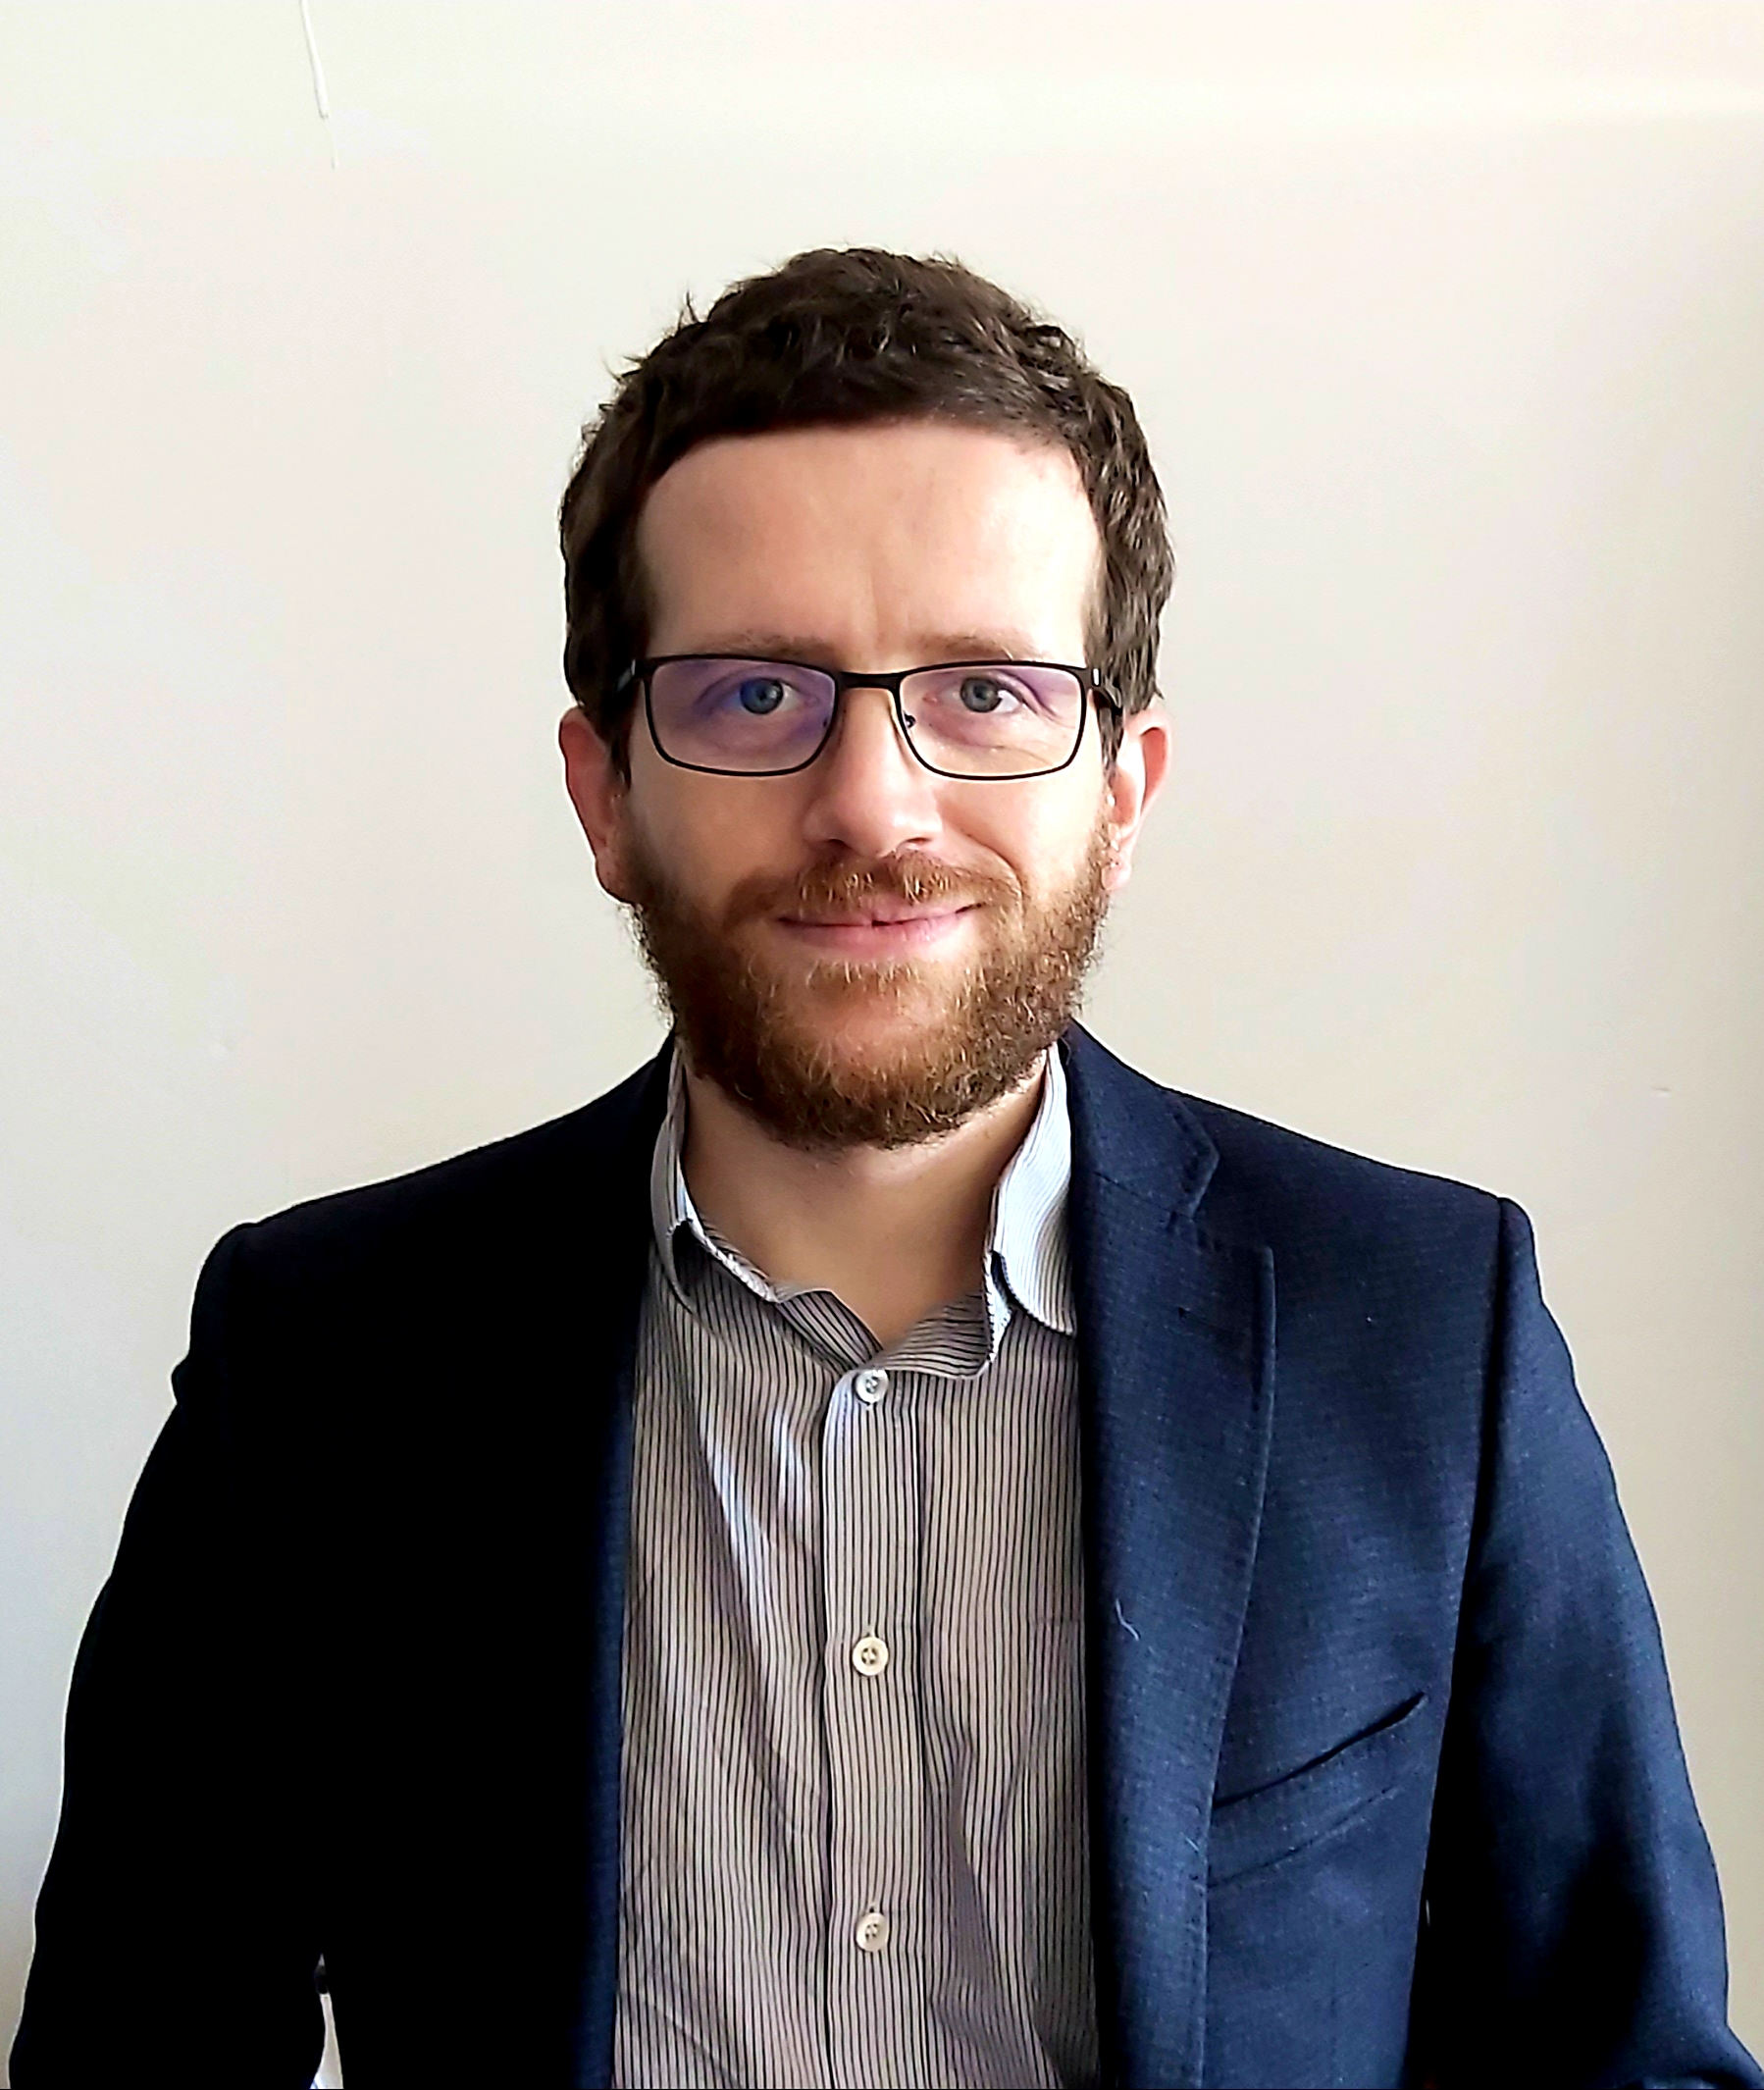
\includegraphics[width = 0.4 \textwidth]{./start/pic.jpg}
\end{center}

\hypertarget{personal-details}{%
\section*{Personal details}\label{personal-details}}

\begin{itemize}
\tightlist
\item
  \emph{work adress}: prof. St.~Łojasiewicza 11, 30-348 Kraków, Poland
  (room B-2-25)
\item
  \emph{cell phone number}: (+48) 728 364 517
\item
  \emph{e-mail}:
  \href{mailto:kacper.topolnicki@uj.edu.pl}{\nolinkurl{kacper.topolnicki@uj.edu.pl}}
\end{itemize}

\hypertarget{education}{%
\section*{Education}\label{education}}

\begin{itemize}
\tightlist
\item
  \textbf{2014}

  \begin{itemize}
  \tightlist
  \item
    Ph.D.~- Physics
  \item
    \emph{institution}: Faculty of Physics, Astronomy and Applied
    Computer Science of the Jagiellonian University
  \item
    \emph{description}: My thesis titled: ``The two-nucleon and
    three-nucleon systems in three dimensions'' was successfully
    defended on the 23 of September 2014. Subsequently I was awarded a
    Ph.D. degree in physics on 25 September 2014 after the positive
    decision of the Faculty of Physics, Astronomy and Applied Computer
    Science council.
  \end{itemize}
\item
  \textbf{2011-2012}

  \begin{itemize}
  \tightlist
  \item
    \(\approx 0.5\) year Internship at the Institute of Nuclear Physics
    in Jülich
  \item
    \emph{institution}: Institut für Kernphysik, Forschungszentrum
    Jülich, Germany
  \item
    \emph{description}: My half year stay at the interdisciplinary
    research center in Jülich gave me the possibility to have direct
    access to specialists in parallel computing on large computing
    clusters. This was a great opportunity and had a big impact on my
    research.
  \end{itemize}
\item
  \textbf{2010-2014}

  \begin{itemize}
  \tightlist
  \item
    International PhD Studies
  \item
    \emph{institution}: Faculty of Physics, Astronomy and Applied
    Computer Science of the Jagiellonian University
  \item
    \emph{description}: On my second year of regular PhD studies I
    switched over to the
    \href{https://fais.uj.edu.pl/applied-nuclear-physics-and-innovative-technologies}{International
    PhD Studies in Applied Nuclear Physics and Innovative Technologies}.
    The studies lasted for four years. My chosen topic ``Few-nucleon
    fusion reactions'' was being supervised of professor Jacek Golak.
  \end{itemize}
\item
  \textbf{2009-2014}

  \begin{itemize}
  \tightlist
  \item
    Ph.D.~studies in Physics
  \item
    \emph{institution}: Faculty of Physics, Astronomy and Applied
    Computer Science of the Jagiellonian University
  \item
    \emph{description}: PhD studies in Nuclear Physics under the
    supervision of professor Jacek Golak. My research was focused on the
    description of few (two, three) nucleon systems. The character of my
    work was theoretical and included the development of effective
    implementations of numerical calculations on large computing
    clusters (JUQUEEN at the Jülich Supercomputing Centre). A large
    portion of my efforts were focused on developing consistent methods
    for treating the complicated algebraic expressions that arise in the
    calculations. The development of these methods was made possible
    with the use of symbolic programming within the
    \href{https://www.wolfram.com/mathematica/}{Mathematica} system.
  \end{itemize}
\item
  \textbf{2009}

  \begin{itemize}
  \tightlist
  \item
    M.Sc - Physics
  \item
    \emph{institution}: Faculty of Physics, Astronomy and Applied
    Computer Science of the Jagiellonian University
  \item
    \emph{description}: In 2009 I finished my five year studies in
    physics (majored in theoretical physics). My masters thesis titled:
    ``Lattice models of chiral liquid crystal phases in Monte Carlo
    simulations'' was written under the supervision of professor Lech
    Longa.
  \end{itemize}
\item
  \textbf{2004-2009}

  \begin{itemize}
  \tightlist
  \item
    Studies in Physics
  \item
    \emph{description}: Faculty of Physics, Astronomy and Applied
    Computer Science of the Jagiel- lonian University
  \item
    \emph{institution}: In 2004 I started ``Studies in Mathematics and
    Natural Sciences''. I chose to specialize in theoretical physics.
  \end{itemize}
\end{itemize}

\hypertarget{positions}{%
\section*{Positions}\label{positions}}

\begin{itemize}
\tightlist
\item
  \textbf{2020-}

  \begin{itemize}
  \tightlist
  \item
    {[}current position{]} adiunkt (english equivalent: assistant
    professor) at the Institute of Physics, Jagiellonian University,
    Kraków, Poland
  \end{itemize}
\item
  \textbf{2017-2020}

  \begin{itemize}
  \tightlist
  \item
    {[}3 years{]} asystent naukowy (english equivalent: research
    assistant) at the Institute of Physics, Jagiellonian University,
    Kraków, Poland
  \end{itemize}
\item
  \textbf{2014-2017}

  \begin{itemize}
  \tightlist
  \item
    {[}2015, \(\approx\) 0.5 year{]} post-doc at Texas A\&M University
    Commerce
  \item
    various grants (more information in \textbf{Grants} section)
  \end{itemize}
\item
  \textbf{2009-2014}

  \begin{itemize}
  \tightlist
  \item
    {[}2009-2014, 5 years{]} PhD student at the Institute of Physics
    (nuclear theory, few body systems), Jagiellonian University, Kraków,
    Poland
  \item
    {[}2010-2014, 4 years{]} stipend from the
    \href{https://fais.uj.edu.pl/applied-nuclear-physics-and-innovative-technologies}{International
    PhD Studies in Applied Nuclear Physics and Innovative Technologies}
  \item
    {[}2011-2012, \(\approx\) 0.5 year{]} internship at the
    \href{https://www.fz-juelich.de/ikp/EN/Home/home_node.html}{Nuclear
    Physics Institute (IKP)} in Forschungszentrum Jülich, Germany
  \end{itemize}
\end{itemize}

\hypertarget{grants}{%
\section*{Grants}\label{grants}}

\begin{itemize}
\tightlist
\item
  principal investigator

  \begin{itemize}
  \tightlist
  \item
    {[}2017-2020, 3 years{]} SONATA 11

    \begin{itemize}
    \tightlist
    \item
      \emph{funding agency}: National Science Center, Poland
    \item
      \emph{grant number}: DEC-2016/21/D/ST2/01120
    \item
      \emph{title}: ``Development of analytical and numerical
      computation techniques related to few-nucleon systems''
    \end{itemize}
  \item
    {[}2014-2016, 2 years{]} PRELUDIUM 6

    \begin{itemize}
    \tightlist
    \item
      \emph{funding agency}: National Science Center, Poland
    \item
      \emph{grant number}: DEC-2013/11/N/ST2/03733
    \item
      \emph{title}: ``Development of techniques using a three
      dimensional representation of nucleonic degrees of freedom in
      few-nucleon bound and scattering state calculations''
    \end{itemize}
  \end{itemize}
\item
  co-executor

  \begin{itemize}
  \tightlist
  \item
    {[}2017{]} HARMONIA 8

    \begin{itemize}
    \tightlist
    \item
      \emph{funding agency}: National Science Center, Poland
    \item
      \emph{grant number}: DEC-2016/22/M/ST2/00173
    \item
      \emph{title}: ``Utilizing consistent chiral nuclear potentials and
      electroweak currents in order to describe three nucleon reactions
      and properties of nuclei''
    \end{itemize}
  \item
    {[}2014-2016{]} HARMONIA 5

    \begin{itemize}
    \tightlist
    \item
      \emph{funding agency}: National Science Center, Poland
    \item
      \emph{grant number}: DEC-2013/10/M/ST2/00420
    \item
      \emph{title}: ``Investigation of the properties of light nuclei
      and three body processes based on chiral nuclear potentials)''
    \end{itemize}
  \end{itemize}
\end{itemize}

\hypertarget{skills-and-experience}{%
\section*{Skills and experience}\label{skills-and-experience}}

\begin{itemize}
\tightlist
\item
  academic interests

  \begin{itemize}
  \tightlist
  \item
    few body systems
  \item
    nuclear theory
  \item
    numerical calculations
  \item
    teaching
  \end{itemize}
\item
  languages

  \begin{itemize}
  \tightlist
  \item
    Polish (native)
  \item
    English (CAE - 2003, CPE - 2006)
  \end{itemize}
\item
  programming

  \begin{itemize}
  \tightlist
  \item
    parallel computing on large computing clusters using MPI, OPENMP
  \item
    Wolfram Language, Fortran (different flavours), python (different
    flavours), c, bash
  \item
    other programming languages with less proficiency
  \end{itemize}
\item
  software

  \begin{itemize}
  \tightlist
  \item
    linux
  \item
    standard Linux tools
  \item
    LaTeX, gnuplot, Mathematica
  \end{itemize}
\end{itemize}

\section{External links}

\tightlist
\item list of publications (WOS, I 2021) (\href{https://kacpertopol.github.io/cv/0pl.html}{link})
\item list of talks (\href{https://kacpertopol.github.io/cv/00pl.html}{link})

  \begin{itemize}
  \tightlist
  \item
    few body systems
  \item
    nuclear theory
  \item
    numerical calculations
  \item
    teaching
  \end{itemize}
\item
  languages

\hypertarget{publications-wos-i-2021}{%
\section*{\texorpdfstring{\href{./0pl.html}{Publications (WOS, I
2021)}}{Publications (WOS, I 2021)}}\label{publications-wos-i-2021}}

\hypertarget{talks}{%
\section*{\texorpdfstring{\href{./00pl.html}{Talks}}{Talks}}\label{talks}}

\hypertarget{other-interests}{%
\section*{Other interests}\label{other-interests}}

\begin{itemize}
\tightlist
\item
  \href{https://kacpertopol.github.io/myblog/}{my blog}
\item
  \emph{music}: Tom Waits, Gelnn Gould
\item
  \emph{sport}: skiing, windsurfing, air-soft
\end{itemize}
\end{document}
